\documentclass[12pt]{article}
\usepackage{bookmark}
% --- Paquetes para el diseño ---
\usepackage[utf8]{inputenc}
\usepackage{lmodern}
\usepackage[spanish,provide=*]{babel}
\usepackage[margin=1.5cm,top=2cm, bottom=3cm,headheight=0pt, headsep=0.5cm]{geometry}
\usepackage{graphicx}
\usepackage{float}
\usepackage{xcolor}
\usepackage{tcolorbox} % Para los cuadros grises redondeados
\tcbuselibrary{breakable}
\usepackage{array}
\usepackage{hyperref}
\usepackage{fancyhdr}   % Para el encabezado de las páginas siguientes
\usepackage{titlesec}   % Para personalizar los títulos
\usepackage{enumitem}
\usepackage{listings}
\usepackage{caption}
\usepackage{amssymb} % Necesario para los símbolos N y Z
\usepackage{amsmath} % Recomendado para texto dentro de fórmulas

% Configuración para quitar "Listing #:"
\DeclareCaptionFormat{listing}{\textbf{#3}}

% --- ESTILO PARA C (Multihilos) ---
\lstdefinestyle{estiloC}{
    language=C,
    basicstyle=\ttfamily\small,
    keywordstyle=\color{blue}\bfseries,
    commentstyle=\color{green!50!black},
    stringstyle=\color{orange},
    numbers=left,
    numberstyle=\tiny\color{green!50!black},
    stepnumber=1,
    numbersep=8pt,
    frame=single,
    rulecolor=\color{black},
    breaklines=true,
    showstringspaces=false,
    tabsize=4,
    keepspaces=true,
    columns=flexible,
    xleftmargin=20pt,
    morekeywords={NULL, sendto, recvfrom, bzero, printf, close, exit, perror, strlen, memset, bind},
    extendedchars=true,
    literate={á}{{\'a}}1 {é}{{\'e}}1 {í}{{\'i}}1 {ó}{{\'o}}1 {ú}{{\'u}}1 {ñ}{{\~n}}1
}

% --- Configuración de los cuadros (Estilo idéntico al documento) ---
\tcbset{
    estilo_practica/.style={
        colback=gray!20,      % Color de fondo gris claro
        colframe=gray!20,     % Color del borde (igual al fondo)
        arc=12pt,             % Redondeo de las esquinas
        boxrule=0pt,
        left=15pt, right=15pt, top=8pt, bottom=8pt,
        halign=center,        % Alineación del texto dentro
        fonttitle=\bfseries\large,
        coltitle=black,
        before skip=10pt,
        after skip=10pt
    }
}

% --- Configuración de Colores ---
\definecolor{azul_unam}{RGB}{31, 78, 121} % Azul similar al de la imagen

% --- Estilo de los Títulos (Azul y Negrita) ---
\titleformat{\section}
  {\color{azul_unam}\normalfont\bfseries\centering}{}{0pt}{}
  
\titleformat{\subsection}
  {\color{azul_unam}\normalfont\bfseries}{}{0pt}{\thesubsection\ }

\titleformat{\subsubsection}
  {\color{azul_unam}\normalfont\bfseries}{}{0pt}{\thesubsubsection\ }

% --- Configuración del Encabezado (Páginas Siguientes) ---
\pagestyle{fancy}
\fancyhf{}
\renewcommand{\headrulewidth}{1pt}
\renewcommand{\headrule}{\hbox to\headwidth{\color{azul_unam}\leaders\hrule height \headrulewidth\hfill}}

\fancyhead[L]{
    \small 
\includegraphics[height=1.25cm]{logo_fi.png} % Ajusta el nombre de tu archivo
    \quad Facultad de Ingeniería UNAM
}
\fancyhead[R]{\small \textit{Sistemas Distribuidos}}
\fancyfoot[C]{\thepage}

\setlength{\headheight}{50.95274pt}
\addtolength{\topmargin}{-22.95274pt}
\setlength{\parindent}{0pt}

% --- CUERPO DEL DOCUMENTO ---
\begin{document}
\pagestyle{empty} % Quitar números de página en la portada

\vspace*{-2.5cm}
% --- Encabezado con Logos ---
\begin{table}[h]
\centering
\begin{tabular}{m{3cm} m{11cm} m{3cm}}
    
\includegraphics[width=3cm]{logo_unam.png} & 
    \centering
    \textcolor[rgb]{0.2, 0.4, 0.6}{\textbf{\Large Primer Parcial}} \\[0.2cm]
    \textbf{\LARGE Examen Práctico} \\[0.2cm]
    \large Prof. Carmen Lucia Bustillo Hernández \\
    \texttt{Universidad Nacional Autónoma de México} \\[0.1cm]
    Fecha de Entrega: 9 de Abril de 2026 &
    \centering
    
\includegraphics[width=2.85cm]{logo_fi.png} \\ 
\end{tabular}
\end{table}

\vspace{-0.5cm}
% --- Títulos Centrales ---
\begin{flushleft}
    \textbf{Nombre:} Cortez Rios Enrique Yoab \\[0.25cm]
    \textbf{No. cuenta:} 317302992 \\[0.25cm]
    \textbf{Firma:} \\[0.25cm]
    \textbf{Nombre:} Mendoza Gonzáles Mario\\[0.25cm]
    \textbf{No. cuenta:} \\[0.25cm]
    \textbf{Firma:}
\end{flushleft}
\vspace{0.5cm}

% --- Cuadro: Instrucciones ---
\begin{tcolorbox}[estilo_practica]
    \begin{center}
        \textbf{Instrucciones}
    \end{center}
    \begin{enumerate}
        \item Lea su examen cuidadosamente. Ponga cuidado a los detalles.
        \item Para la realización de su examen se requiere un equipo de dos personas.
        \item La evaluación consiste en la demostración presencial del problema planteado, utilizando dos computadoras conectadas mediante cable de red.
        \item Presentar pseudocódigo, diagrama de flujo y código respectivamente.
        \item Presentar la documentación correspondiente a la base de datos.
        \item El contenido que esté fuera de contexto del tema del examen será ANULADO.
    \end{enumerate}
\end{tcolorbox}

% --- Cuadro: Objetivos Específicos ---
\begin{tcolorbox}[estilo_practica]
    \begin{center}
        \textbf{Criterios de Evaluación}
    \end{center}
    \begin{enumerate}
        \item Modelo Entidad-Relación y Normalización de la Base de Datos = 12.5 pts.
        \item Pseudocódigo y diagrama de flujo = 12.5 pts. 
        \item Código de la aplicación = 25 pts.
    \end{enumerate}
\end{tcolorbox}

\newpage % --- Segunda Pagina
\pagestyle{fancy}

\section{\large 1. Problemas}
\subsection{Problema 1}
Crear una aplicación (Utilizando sockets de tipo de flujo como datagrama y TCP) que desde la máquina cliente solicite a un servidor consultas sobre la base de datos (Universidad.xls). Normalice a la 4FN respectivamente la base de datos proporcionada. La aplicación debe consultar, modificar, eliminar o actualizar los registros de la base de datos respectivamente desde el cliente. Para el desarrollo de este problema, puede utilizar: \textbf{50 pts.}

\begin{itemize}
    \item Un gestor de bases de datos (MySQL, PostgreSQL, entre otros).
    \item Gestión de la base de datos mediante archivos de texto.
\end{itemize}

\textbf{Nota:} Insertar todos los registros que vienen en el archivo Universidad.xls para realizar las consultas.

\subsection{Solución}

Para poder levantar la base de datos por medio de archivos de texto, lo principal es normalizar la base del archivo "Universidad.xls". Posterior a esto, debemos migrar los datos que contiene originalmente a la nueva estructura normalizada que se muestra a continuación:

\begin{figure}[H]
    \centering
    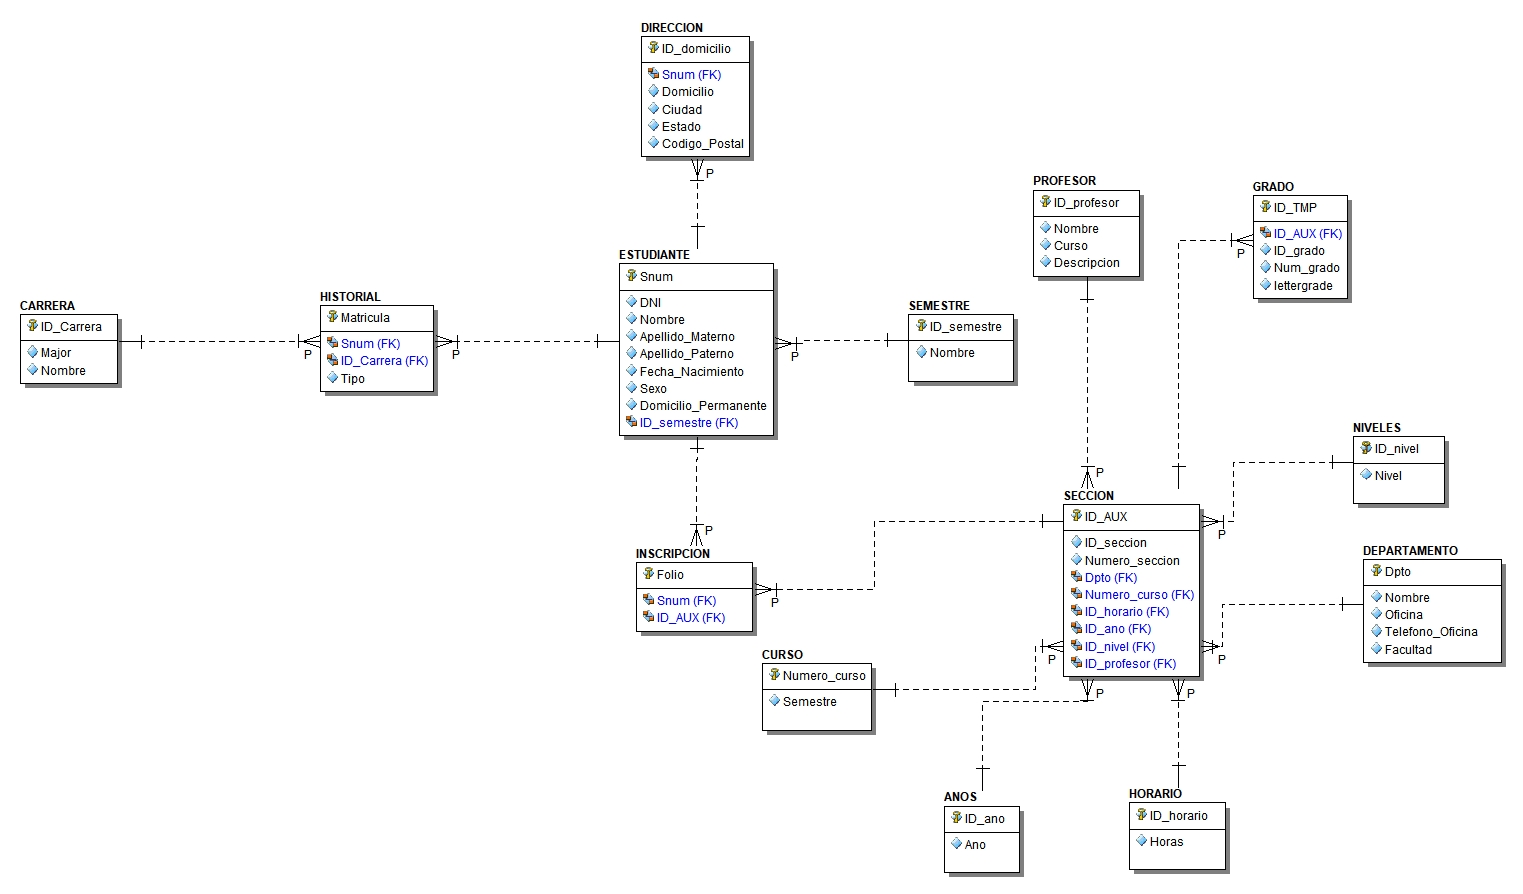
\includegraphics[width=1.0\textwidth]{Diagrama Entidad-Relacion.jpeg} 
    \caption{Diagrama Entidad-Relación}
\end{figure}

Con esto podemos identificar varios elementos importantes: son 14 tablas, las cuales debemos crear como archivos y llenarlas con sus respectivos datos.

\subsubsection{Tabla Estudiantes}
Esta tabla almacena los 20 registros de los estudiantes, su semestre y el domicilio permanente. Esto evita agregar registros vacíos dentro de la tabla dirección, además de ser atributos intrínsecos del estudiante.

\begin{figure}[H]
    \centering
    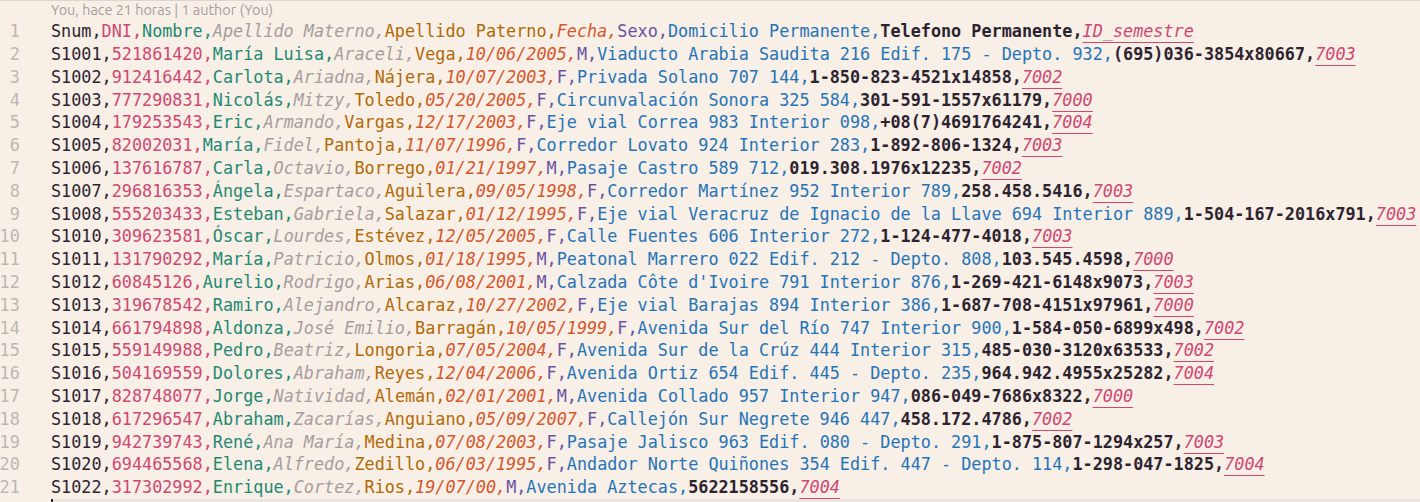
\includegraphics[width=1.0\textwidth]{Estudiantes.png} 
    \caption*{Tabla 1. Estudiante}
\end{figure}

\subsubsection{Tabla Dirección}
Esta tabla almacena la dirección actual del estudiante, la cual es más propensa a ser cambiada y por eso no se agrega directamente a la tabla de estudiantes (a diferencia de su domicilio permanente).

\begin{figure}[H]
    \centering
    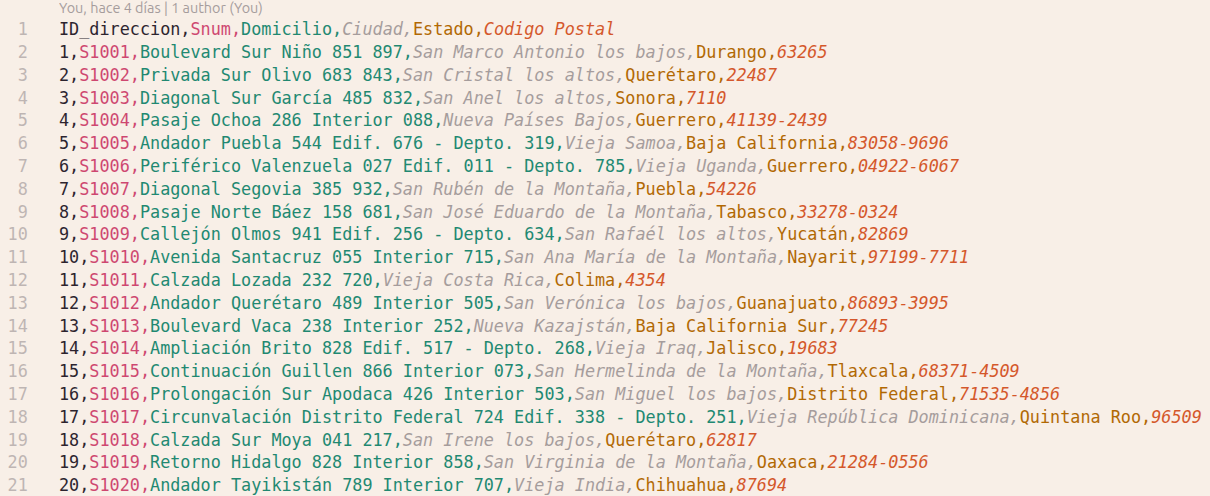
\includegraphics[width=1.0\textwidth]{Direccion.png} 
    \caption*{Tabla 2. Dirección}
\end{figure}

\subsubsection{Tabla Carrera}
La tabla carrera almacena los nombres de cada carrera. Debido a que un estudiante puede cursar una o más carreras, la relación es de muchos a muchos. Esto obliga a generar una tabla intermedia entre el estudiante y las carreras, que se llamará historial.

\begin{figure}[H]
    \centering
    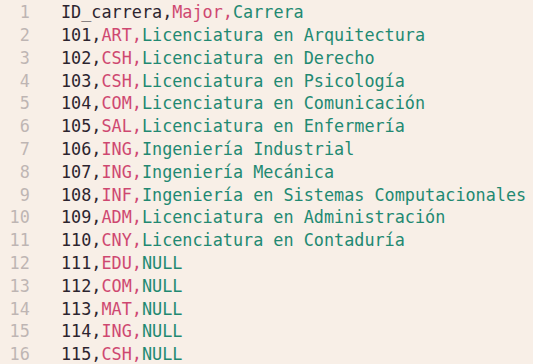
\includegraphics[width=0.40\textwidth]{Carrera.png} 
    \caption*{Tabla 3. Carrera}
\end{figure}

\subsubsection{Tabla Historial}
Esta es la tabla intermedia que se genera entre el estudiante y el catálogo de carreras. Si un registro tiene más de una llave, significa que el alumno cursa más de una carrera.

\begin{figure}[H]
    \centering
    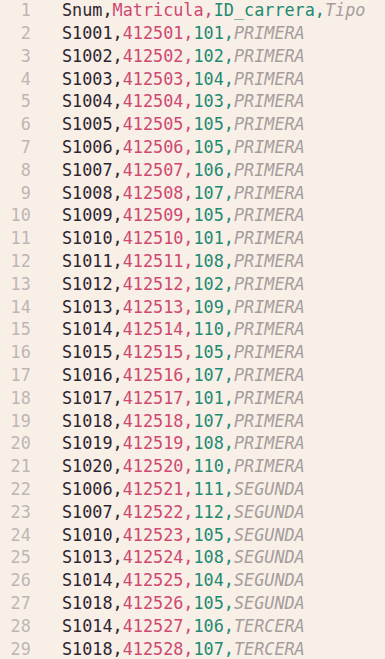
\includegraphics[width=0.32\textwidth]{Historial.png} 
    \caption*{Tabla 4. Historial}
\end{figure}

\subsubsection{Tabla Inscripción}
Esta tabla es el producto de la relación entre el estudiante y la sección en la que está inscrito. Al ser una relación de muchos a muchos, la llamamos inscripción, pues un estudiante puede inscribir una o varias secciones.

\begin{figure}[H]
    \centering
    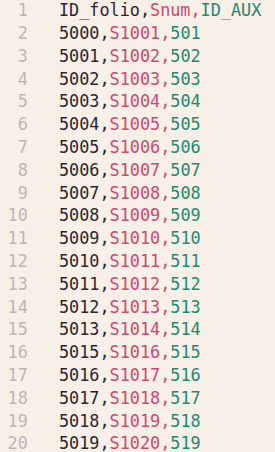
\includegraphics[width=0.28\textwidth]{Inscripcion.png} 
    \caption*{Tabla 5. Inscripción}
\end{figure}

\subsubsection{Tabla Sección}
Esta tabla es la que almacena el registro de la sección inscrita, junto con el profesor y el departamento que la imparte, además de su calificación definida.

\begin{figure}[H]
    \centering
    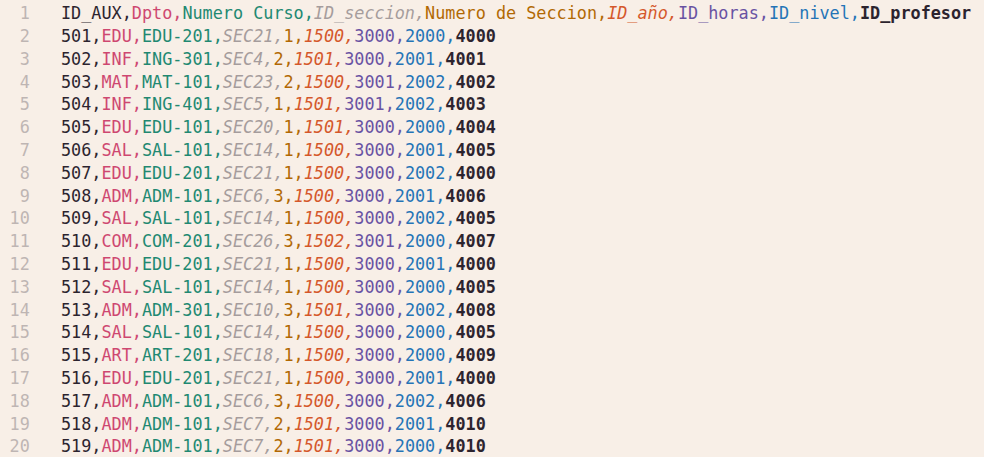
\includegraphics[width=0.75\textwidth]{Seccion.png} 
    \caption*{Tabla 6. Sección}
\end{figure}

\subsubsection{Tabla Profesor}
La tabla profesor almacena el nombre, el curso y una breve descripción de la asignatura que imparte el docente en una o varias secciones.

\begin{figure}[H]
    \centering
    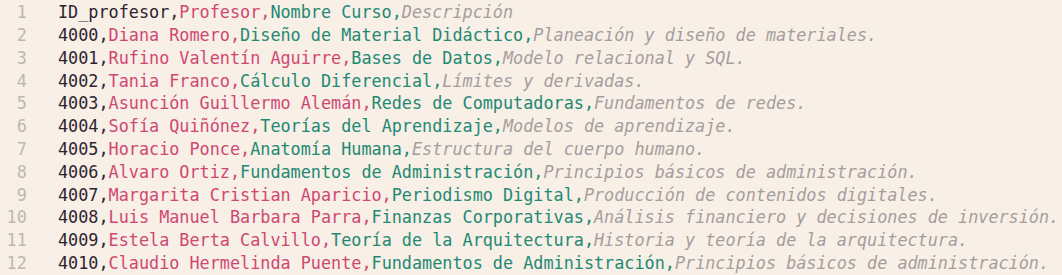
\includegraphics[width=1.0\textwidth]{Profesor.png} 
    \caption*{Tabla 7. Profesor}
\end{figure}

\subsubsection{Tabla Departamento}
El departamento contiene los nombres de cada uno, su abreviatura, un teléfono de oficina y la facultad a la que pertenece la sección.

\begin{figure}[H]
    \centering
    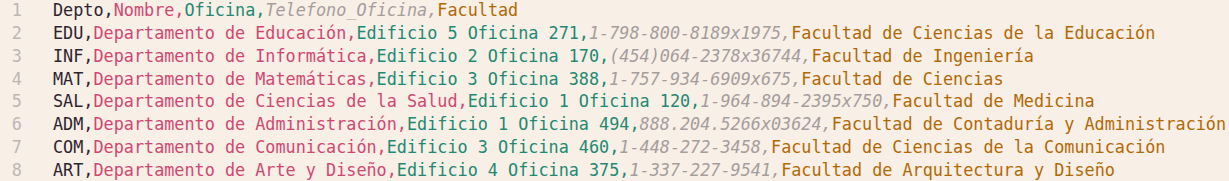
\includegraphics[width=1.0\textwidth]{Departamento.png} 
    \caption*{Tabla 8. Departamento}
\end{figure}

\subsubsection{Tabla Niveles}
Esta tabla solo almacena el nivel en el que se impartió la sección.

\begin{figure}[H]
    \centering
    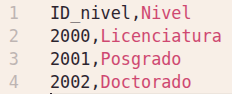
\includegraphics[width=0.35\textwidth]{Niveles.png} 
    \caption*{Tabla 9. Niveles}
\end{figure}

\newpage
\subsubsection{Tabla Horario}
La tabla guarda el número de horas en las que se imparte una sección.

\begin{figure}[H]
    \centering
    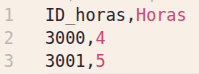
\includegraphics[width=0.25\textwidth]{Horario.png} 
    \caption*{Tabla 10. Horario}
\end{figure}

\subsubsection{Tabla Grado}
La tabla grado almacena la calificación obtenida en una sección.

\begin{figure}[H]
    \centering
    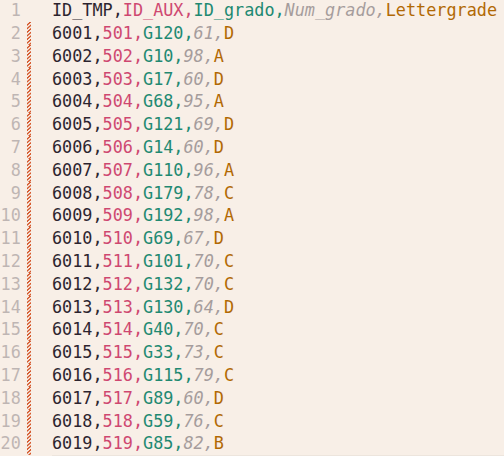
\includegraphics[width=0.40\textwidth]{Grado.png} 
    \caption*{Tabla 11. Grado}
\end{figure}

\subsubsection{Tabla Curso}
La tabla curso almacena la estación del año en la que se imparte la sección y el salón asignado.

\begin{figure}[H]
    \centering
    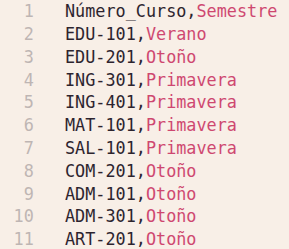
\includegraphics[width=0.30\textwidth]{Curso.png} 
    \caption*{Tabla 12. Curso}
\end{figure}

\subsubsection{Tabla Años}
La tabla años solo almacena el año en el que se impartió la sección.

\begin{figure}[H]
    \centering
    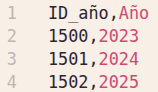
\includegraphics[width=0.25\textwidth]{Años.png} 
    \caption*{Tabla 13. Años}
\end{figure}

\subsubsection{Tabla Semestre}
Esta tabla solo almacena el semestre en el que se encuentra el estudiante.

\begin{figure}[H]
    \centering
    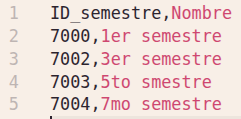
\includegraphics[width=0.35\textwidth]{Semestre.png} 
    \caption*{Tabla 14. Semestre}
\end{figure}

\begin{itemize}
    \item \textbf{Estructura del Cliente}
\end{itemize}

El cliente no contiene nada de lógica ni verificación; esto se realiza exclusivamente en el servidor, el cual también se encarga de reportar los errores al cliente. Para que el usuario pueda interactuar correctamente con la base de datos, debemos sincronizar nuestras peticiones con los parámetros que necesita el servidor para poder realizar de manera exitosa las consultas, inserciones, eliminaciones y actualizaciones. \\
Para que el cliente tenga interacción con el servidor, le agregamos un pequeño submenú que se encarga de indicarle qué comandos son posibles de solicitar. Al utilizar cadenas de texto para interpretar las instrucciones, nos apoyamos en funciones de token o búsqueda de coincidencias para saber si el usuario solicita algún comando en específico.

%Inicia el codigo C del cliente
\begin{lstlisting}[style=estiloC ,title={Código 1. Cliente TCP (MAIN)}]
#include <stdio.h>
#include <stdlib.h>
#include <string.h>
#include <unistd.h>
#include <sys/socket.h>
#include <arpa/inet.h>

#define IP_SERVIDOR "192.168.1.20" // Esta es la ip del servidor 
#define PUERTO 3000
#define TAM_MAX 1024

void realizar_consulta(int sock);
void realizar_insercion(int sock);
void realizar_eliminacion(int sock);
void realizar_actualizacion(int sock);

int main() {
    int sock = 0;
    struct sockaddr_in serv_addr;
    char buffer[TAM_MAX];

    printf("[1] Creando socket TCP...\n");
    if ((sock = socket(AF_INET, SOCK_STREAM, 0)) < 0) return -1;
    serv_addr.sin_family = AF_INET;
    serv_addr.sin_port = htons(PUERTO);
    if (inet_pton(AF_INET, IP_SERVIDOR, &serv_addr.sin_addr) <= 0) return -1;

    printf("[2] Conectando al servidor...\n");
    if (connect(sock, (struct sockaddr *)&serv_addr, sizeof(serv_addr)) < 0) return -1;

    bzero(buffer, TAM_MAX);
    recv(sock, buffer, TAM_MAX, 0);
    printf("\n[Mensaje Inicial del Servidor]: %s", buffer);

    // --- BUCLE INTERACTIVO ---
    while(1) {
        printf("\n===============================================================================\n");
        printf(" COMANDOS ACTIVOS: CONSULTA | INSERCION | ELIMINACION | ACTUALIZACION | OFF |\n");
        printf("=============================================================================\n");
        printf("Tu mensaje (Comando): ");
        
        bzero(buffer, TAM_MAX);
        fgets(buffer, TAM_MAX, stdin);
        buffer[strcspn(buffer, "\n")] = 0;

        if (strstr(buffer, "OFF") != NULL) {
            printf("[!] Cerrando cliente...\n");
            send(sock, "OFF", 3, 0); 
            break;
        }
        else if (strstr(buffer, "CONSULTA") != NULL) {
            realizar_consulta(sock);
        }
        else if(strstr(buffer, "INSERCION") != NULL)
        {
            realizar_insercion(sock);
        }
        else if(strstr(buffer, "ELIMINACION") != NULL)
        {
            realizar_eliminacion(sock);
        }
        else if(strstr(buffer, "ACTUALIZACION") != NULL)
        {
            realizar_actualizacion(sock);
        }else {
            printf("[-] Comando no reconocido. Escribe: CONSULTA, INSERCION, ACTUALIZACION, ELIMINACION o OFF.\n");
        }
    }

    close(sock);
    printf("\nDesconectado exitosamente.\n");
    return 0;
}
\end{lstlisting}

Se desarrolla la función consulta, que es una de las operaciones más usadas dentro de una base de datos. Para que esta sea procesada por el servidor, el cliente debe enviar 3 cosas:
\begin{itemize}
    \item \textbf{Número de tabla:} El identificador de la tabla que se consulta dentro de la base.
    \item \textbf{Llave:} Es el tipo de consulta que se realiza (total, parcial o único).
    \begin{enumerate}
        \item \textbf{full:} Revisará toda la tabla y la regresa completa.
        \item \textbf{low:} Revisa toda la tabla pero retorna solo los atributos que escoja el cliente.
        \item \textbf{ID:} Es el identificador único de cada registro. Si existe, regresa la consulta con los parámetros que define visualizar el cliente.
    \end{enumerate} 
    \item \textbf{Parámetros:} Es una cadena de bits que indica qué atributos de la tabla consultada se desean observar ('1' es para visualizarlo y '0' es para ignorarlo). Por lo tanto, esta cadena de texto es diferente para cada tabla que se encuentra dentro de la base de datos.
\end{itemize}

Al obtener estos datos por medio del teclado, debemos concatenar las respuestas con una barra vertical "|" (o el separador definido) para que el servidor pueda descomponerlo después y verificar si la petición es correcta. En caso de que falle algún dato o parámetro, el mismo servidor regresará el error producido; de lo contrario, se entra en un bucle de comunicación para poder transferir los datos del servidor al cliente. El cliente tendrá un archivo llamado \texttt{consulta.csv} en el que guardará la información obtenida (el contenido se sobrescribirá cada vez que se haga una nueva consulta).

\begin{lstlisting}[style=estiloC ,title={Código 2. Cliente TCP (CONSULTA)}]
void realizar_consulta(int sock) {
    char tabla[10], llave[50], mascara[50], paquete_envio[TAM_MAX], respuesta_servidor[TAM_MAX];
    printf("\n\t--- MODO CONSULTA ---\n");
    printf("[ESTUDIANTE,0]\t\t[DIRECCION,1]\n[CARRERA,2]\t\t[HISTORIAL,3]\n[INSCRIPCION,4]\t\t[SECCION,5]\n[PROFESOR,6]\t\t[DEPARTAMENTO,7]\n");
    printf("[NIVELES,8]\t\t[HORARIO,9]\n[GRADO,10]\t\t[CURSO,11]\n[ANOS,12]\t\t[SEMESTRE,13]\n");
    printf("Ingresa el numero de tabla (0-13): ");
    fgets(tabla, sizeof(tabla), stdin); tabla[strcspn(tabla, "\n")] = 0;
    printf("Ingresa la llave a buscar ('full', 'low' o ID): ");
    fgets(llave, sizeof(llave), stdin); llave[strcspn(llave, "\n")] = 0;
    printf("Ingresa la mascara de parametros (Bits 1/0): ");
    fgets(mascara, sizeof(mascara), stdin); mascara[strcspn(mascara, "\n")] = 0;

    sprintf(paquete_envio, "1|%s|%s|%s", tabla, llave, mascara);
    send(sock, paquete_envio, strlen(paquete_envio), 0);

    // --- NUEVA LOGICA DE RECEPCION ---
    bzero(respuesta_servidor, sizeof(respuesta_servidor));
    recv(sock, respuesta_servidor, sizeof(respuesta_servidor), 0);
    // Verificamos si el servidor activó el modo de envío por renglones
    if (strncmp(respuesta_servidor, "CANTIDAD|", 9) == 0) {
        // Extraemos el número que viene después de "CANTIDAD|"
        int total_filas = atoi(respuesta_servidor + 9);
        if(strstr(llave, "full") != NULL || strstr(llave, "FULL") != NULL || strstr(llave, "low") != NULL || strstr(llave, "LOW") != NULL ) total_filas--;
        printf("\n--- RESULTADOS DE LA BD (%d registros) ---\n", total_filas);
        // Abrimos el archivo en donde se guardara la consulta
        FILE *archivo = fopen("./consulta.csv", "w");
        // Le decimos al servidor: "Estoy listo, manda el primero" (ACK)
        send(sock, "ACK", 3, 0);
        // Bucle para recibir uno por uno
        for(int i = 0; i < total_filas; i++) {
            bzero(respuesta_servidor, sizeof(respuesta_servidor));
            recv(sock, respuesta_servidor, sizeof(respuesta_servidor), 0);
            
            // Imprimimos el renglón recibido
            printf("[%d]: %s\n", i, respuesta_servidor);
            fprintf(archivo,"%s\n",respuesta_servidor);
            // Confirmamos recepción (ACK) para que el servidor mande el siguiente
            send(sock, "ACK", 3, 0);
        }
        printf("----------------------------------------\n");
        fclose(archivo);
    } else {
        // Si no era "CANTIDAD|", significa que es un Error o un "No se encontraron registros"
        printf("\n[Servidor]: %s\n", respuesta_servidor);
    }
}
\end{lstlisting}

La función de inserción solicita solo 1 parámetro inicial para enviar al servidor, el cual retornará la cantidad de columnas o registros que se deben llenar para poder ser insertados en la tabla. El mismo servidor verifica que todos los campos estén completos (de lo contrario no podrá insertarlo), además de validar que la llave primaria ingresada no se repita en la tabla. Si el servidor retorna un valor válido, empieza el proceso de captura de los datos solicitados.

\begin{lstlisting}[style=estiloC ,title={Código 3. Cliente TCP (INSERCION)}]
void realizar_insercion(int sock)
{
    char tabla[10], paquete_envio[TAM_MAX], respuesta_servidor[TAM_MAX];
    char datos_csv[TAM_MAX] = "";
    // Aquí armaremos la fila con comas
    char entrada_temporal[256];
    //El buffer que almacenara lo del teclado

    printf("\n--- MODO INSERCION ---\n");
    printf("Ingresa el numero de tabla (0-13): ");
    fgets(tabla, sizeof(tabla), stdin); tabla[strcspn(tabla, "\n")] = 0;
    // FASE 1: Enviar petición inicial al servidor (Operación 2 | Tabla)
    sprintf(paquete_envio, "2|%s", tabla);
    send(sock, paquete_envio, strlen(paquete_envio), 0);

    // FASE 2: Esperar respuesta del servidor (Debería ser "COLUMNAS|N")
    bzero(respuesta_servidor, sizeof(respuesta_servidor));
    recv(sock, respuesta_servidor, sizeof(respuesta_servidor), 0);

    if (strncmp(respuesta_servidor, "COLUMNAS|", 9) == 0) {
        
        // Extraemos el número de columnas que el servidor contó
        int num_columnas = atoi(respuesta_servidor + 9);
        printf("[*] El servidor verifico la tabla. Se requieren %d columnas.\n", num_columnas);
        printf("--------------------------------------------------\n");
        // Preparamos el inicio del paquete final
        strcpy(datos_csv, "DATOS|");
        // FASE 3: Bucle interactivo pidiendo al usuario dato por dato
        for (int i = 0; i < num_columnas; i++) {
            if (i == 0) {
                printf("Ingrese el dato para la columna %d (LLAVE PRIMARIA): ", i + 1);
            } else {
                printf("Ingrese el dato para la columna %d: ", i + 1);
            }
            
            bzero(entrada_temporal, sizeof(entrada_temporal));
            fgets(entrada_temporal, sizeof(entrada_temporal), stdin);
            entrada_temporal[strcspn(entrada_temporal, "\n")] = 0; // Quitar salto

            // Concatenamos el dato ingresado a nuestra cadena principal
            strcat(datos_csv, entrada_temporal);
            // Si no es la última columna, le agregamos una coma separadora
            if (i < num_columnas - 1) {
                strcat(datos_csv, ",");
            }
        }

        // FASE 4: Enviar la fila completa al servidor
        printf("\n[Enviando paquete]: %s\n", datos_csv);
        send(sock, datos_csv, strlen(datos_csv), 0);

        // FASE 5: Esperar el veredicto final (Exito o Error por llave duplicada)
        bzero(respuesta_servidor, sizeof(respuesta_servidor));
        recv(sock, respuesta_servidor, sizeof(respuesta_servidor), 0);

        printf("[Respuesta del Servidor]: %s\n", respuesta_servidor);

    } else {
        // Si el servidor no respondió "COLUMNAS|", significa que hubo un error (ej. tabla inválida)
        printf("\n[Servidor rechazo la peticion]: %s\n", respuesta_servidor);
    }
}
\end{lstlisting}

Para la función de eliminación, el cliente solo necesita capturar 2 datos:
\begin{enumerate}
    \item \textbf{Número de Tabla:} El identificador de la tabla donde se eliminará el registro.
    \item \textbf{ID único:} La llave primaria del registro en la base de datos.
\end{enumerate}

\begin{lstlisting}[style=estiloC ,title={Código 4. Cliente TCP (ELIMINACION)}]
void realizar_eliminacion(int sock) 
{
    char tabla[10], llave[50], paquete_envio[TAM_MAX], respuesta_servidor[TAM_MAX];
    printf("\n--- MODO ELIMINACION ---\n");
    printf("Ingresa el numero de tabla (0-13): ");
    fgets(tabla, sizeof(tabla), stdin); tabla[strcspn(tabla, "\n")] = 0;
    printf("Ingresa el ID (llave primaria) a eliminar: ");
    fgets(llave, sizeof(llave), stdin); llave[strcspn(llave, "\n")] = 0;
    // FASE 1: Enviamos Operacion(3) | Tabla | Llave
    sprintf(paquete_envio, "3|%s|%s", tabla, llave);
    send(sock, paquete_envio, strlen(paquete_envio), 0);
    // FASE 2: Esperamos la respuesta del servidor
    bzero(respuesta_servidor, TAM_MAX);
    recv(sock, respuesta_servidor, TAM_MAX, 0);
    printf("\n[Respuesta del Servidor]: %s\n", respuesta_servidor);
}
\end{lstlisting}

La función de actualización debe capturar nuevamente lo siguiente:
\begin{enumerate}
    \item \textbf{Número de Tabla:} La tabla en la que se actualizará un registro.
    \item \textbf{ID:} El identificador único del registro que se va a modificar.
\end{enumerate}
Al obtener esto del usuario, se envía la llave para revisar si existe en esa tabla antes de intentar actualizarlo. La respuesta del servidor indicará el número de columnas que contiene esa tabla; de lo contrario, si la llave no existe, no se podrá actualizar el registro.

\begin{lstlisting}[style=estiloC ,title={Código 5. Cliente TCP (ACTUALIZACION)}]
void realizar_actualizacion(int sock) {
    char tabla[10], llave_vieja[50], paquete_envio[TAM_MAX], respuesta_servidor[TAM_MAX];
    char datos_csv[TAM_MAX] = "";
    char entrada_temporal[256];

    printf("\n--- MODO ACTUALIZACION ---\n");
    printf("Ingresa el numero de tabla (0-13): ");
    fgets(tabla, sizeof(tabla), stdin);
    tabla[strcspn(tabla, "\n")] = 0;
    
    printf("Ingresa la llave ORIGINAL del registro a modificar: ");
    fgets(llave_vieja, sizeof(llave_vieja), stdin); llave_vieja[strcspn(llave_vieja, "\n")] = 0;
    // FASE 1: Le enviamos la tabla y la llave vieja al servidor para ver si existe
    sprintf(paquete_envio, "4|%s|%s", tabla, llave_vieja);
    send(sock, paquete_envio, strlen(paquete_envio), 0);

    bzero(respuesta_servidor, TAM_MAX);
    recv(sock, respuesta_servidor, TAM_MAX, 0);
    // FASE 2: Si el servidor responde con las columnas, significa que el registro SI existe
    if (strncmp(respuesta_servidor, "COLUMNAS|", 9) == 0) {
        
        int num_columnas = atoi(respuesta_servidor + 9);
        printf("[*] Registro encontrado. Ingresa los nuevos datos (%d columnas).\n", num_columnas);
        printf("--------------------------------------------------\n");

        strcpy(datos_csv, "DATOS|");
        // FASE 3: Bucle interactivo para armar la nueva fila
        for (int i = 0; i < num_columnas; i++) {
            if (i == 0) {
                printf("NUEVA Llave Primaria (Puede ser la misma '%s'): ", llave_vieja);
            } else {
                printf("NUEVO dato para la columna %d: ", i + 1);
            }
            
            bzero(entrada_temporal, sizeof(entrada_temporal));
            fgets(entrada_temporal, sizeof(entrada_temporal), stdin);
            entrada_temporal[strcspn(entrada_temporal, "\n")] = 0;

            strcat(datos_csv, entrada_temporal); 
            if (i < num_columnas - 1) strcat(datos_csv, ",");
        }

        // FASE 4: Enviar la fila completa
        printf("\n[Enviando actualizacion]: %s\n", datos_csv);
        send(sock, datos_csv, strlen(datos_csv), 0);

        // FASE 5: Recibir éxito o error (ej. si la nueva llave choca con otra)
        bzero(respuesta_servidor, TAM_MAX);
        recv(sock, respuesta_servidor, TAM_MAX, 0);
        printf("[Respuesta del Servidor]: %s\n", respuesta_servidor);

    } else {
        // Si no respondió "COLUMNAS|", es un error (seguramente la llave no existe)
        printf("\n[Servidor rechazo la peticion]: %s\n", respuesta_servidor);
    }
}
\end{lstlisting}

Con esto definido por parte del cliente, el servidor debe solucionar la comunicación entrante, la lectura de los archivos y la identificación de las llaves dentro de las tablas, además de informar sobre los errores internos que no permiten completar la petición del cliente.

%---------------------------- AQUI VA LO DEL PSEUDOCODIGO Y LOS DIAGRAMAS -----------------------------------
\newpage
\begin{itemize}
    \item \textbf{Pseudocódigo (Cliente)}
\end{itemize}

\begin{tcolorbox}[colback=white, colframe=azul_unam, title=Pseudocódigo: Cliente de Base de Datos Distribuida (Completo), breakable]
\begin{small}
\begin{tabbing}
\hspace{0.6cm} \= \hspace{0.6cm} \= \hspace{0.6cm} \= \hspace{0.6cm} \= \hspace{0.6cm} \kill
\textbf{Algoritmo} cliente\_bd \\
\> \textbf{Definir} $sock, total\_filas, num\_columnas \in \mathbb{Z}$ \\
\> \textbf{Definir} $serv\_addr \in sockaddr\_in$ \\
\> \textbf{Definir} $\{ c \in \text{Alfabeto} \}, buffer, respuesta, paquete, datos\_csv, |buffer| = 1024$ \\
\> \textbf{Definir} $ip\_serv \in \text{Alfabeto}, ip\_serv =$ "192.168.1.20" \\
\> \textbf{Definir} $puerto \in \mathbb{N}, puerto = 3000$ \\
\\
\> /* 1. Conexión Inicial TCP */ \\
\> $sock = \text{Crear\_Socket}(\text{AF\_INET}, \text{SOCK\_STREAM})$ \\
\> $\text{Configurar\_Direccion}(serv\_addr, ip\_serv, puerto)$ \\
\> \textbf{SI} $\text{Conectar}(sock, serv\_addr) < 0$ \textbf{ENTONCES} \textbf{SALIR} \\
\> $\text{Recibir}(sock, respuesta)$ \quad // Mensaje de bienvenida \\
\\
\> /* 2. Bucle de Interacción Principal */ \\
\> \textbf{MIENTRAS} (Verdadero) \textbf{HACER} \\
\> \> \textbf{ESCRIBIR} "Comandos (CONSULTA, INSERCION, ELIMINACION, \\
\> \> ACTUALIZACION, OFF): " \\
\> \> \textbf{LEER} $buffer$ \\
\\
\> \> \textbf{CASO} $buffer$ \textbf{SEA}: \\
\> \> \> "OFF": \\
\> \> \> \> $\text{Enviar}(sock, \text{"OFF"})$ \\
\> \> \> \> \textbf{ROMPER\_CICLO} \\
\\
\> \> \> "CONSULTA": \textbf{LLAMAR} realizar\_consulta($sock$) \\
\> \> \> "INSERCION": \textbf{LLAMAR} realizar\_insercion($sock$) \\
\> \> \> "ELIMINACION": \textbf{LLAMAR} realizar\_eliminacion($sock$) \\
\> \> \> "ACTUALIZACION": \textbf{LLAMAR} realizar\_actualizacion($sock$) \\
\> \> \> \textbf{OTRO}: \textbf{ESCRIBIR} "Comando no reconocido" \\
\> \> \textbf{FINCASO} \\
\> \textbf{FINMIENTRAS} \\
\> $\text{Cerrar\_Socket}(sock)$ \\
\textbf{FinAlgoritmo} \\
\\
\textbf{Procedimiento} realizar\_consulta($sock$) \\
\> \textbf{LEER} $tabla, llave, mascara$ \\
\> $paquete = \text{Concatenar}(\text{"1|"}, tabla, \text{"|"}, llave, \text{"|"}, mascara)$ \\
\> $\text{Enviar}(sock, paquete)$ \\
\> $\text{Recibir}(sock, respuesta)$ \\
\> \textbf{SI} $\text{Subcadena}(respuesta, 0, 9) == \text{"CANTIDAD|"}$ \textbf{ENTONCES} \\
\> \> $total\_filas = \text{Convertir\_Entero}(respuesta + 9)$ \\
\> \> $\text{Enviar}(sock, \text{"ACK"})$ \\
\> \> \textbf{PARA} $i=0$ \textbf{HASTA} $total\_filas - 1$ \textbf{HACER} \\
\> \> \> $\text{Recibir}(sock, respuesta)$ \\
\> \> \> \textbf{ESCRIBIR} $respuesta$ \quad // Mostrar fila recibida \\
\> \> \> $\text{Enviar}(sock, \text{"ACK"})$ \\
\> \> \textbf{FINPARA} \\
\> \textbf{SINO} \textbf{ESCRIBIR} $respuesta$ \\
\textbf{FinProcedimiento} \\
\\
\textbf{Procedimiento} realizar\_insercion($sock$) \\
\> \textbf{LEER} $tabla$ \\
\> $\text{Enviar}(sock, \text{"2|"} + tabla)$ \\
\> $\text{Recibir}(sock, respuesta)$ \\
\> \textbf{SI} $\text{Subcadena}(respuesta, 0, 9) == \text{"COLUMNAS|"}$ \textbf{ENTONCES} \\
\> \> $num\_columnas = \text{Convertir\_Entero}(respuesta + 9)$ \\
\> \> $datos\_csv = \text{"DATOS|"}$ \\
\> \> \textbf{PARA} $i=1$ \textbf{HASTA} $num\_columnas$ \textbf{HACER} \\
\> \> \> \textbf{LEER} $dato\_temporal$ \\
\> \> \> $datos\_csv = datos\_csv + dato\_temporal$ \\
\> \> \> \textbf{SI} $i < num\_columnas$ \textbf{ENTONCES} $datos\_csv = datos\_csv + \text{","}$ \\
\> \> \textbf{FINPARA} \\
\> \> $\text{Enviar}(sock, datos\_csv)$ \\
\> \> $\text{Recibir}(sock, respuesta\_final)$ \\
\> \> \textbf{ESCRIBIR} $respuesta\_final$ \\
\> \textbf{SINO} \textbf{ESCRIBIR} $respuesta$ \\
\textbf{FINSI} \\
\textbf{FinProcedimiento} \\
\\
\textbf{Procedimiento} realizar\_eliminacion($sock$) \\
\> \textbf{LEER} $tabla, llave$ \\
\> $paquete = \text{Concatenar}(\text{"3|"}, tabla, \text{"|"}, llave)$ \\
\> $\text{Enviar}(sock, paquete)$ \\
\> $\text{Recibir}(sock, respuesta)$ \\
\> \textbf{ESCRIBIR} $respuesta$ \\
\textbf{FinProcedimiento} \\
\\
\textbf{Procedimiento} realizar\_actualizacion($sock$) \\
\> \textbf{LEER} $tabla, llave\_vieja$ \\
\> $paquete = \text{Concatenar}(\text{"4|"}, tabla, \text{"|"}, llave\_vieja)$ \\
\> $\text{Enviar}(sock, paquete)$ \\
\> $\text{Recibir}(sock, respuesta)$ \\
\> \textbf{SI} $\text{Subcadena}(respuesta, 0, 9) == \text{"COLUMNAS|"}$ \textbf{ENTONCES} \\
\> \> $num\_columnas = \text{Convertir\_Entero}(respuesta + 9)$ \\
\> \> $datos\_csv = \text{"DATOS|"}$ \\
\> \> \textbf{PARA} $i=1$ \textbf{HASTA} $num\_columnas$ \textbf{HACER} \\
\> \> \> \textbf{LEER} $dato\_temporal$ \\
\> \> \> $datos\_csv = datos\_csv + dato\_temporal$ \\
\> \> \> \textbf{SI} $i < num\_columnas$ \textbf{ENTONCES} $datos\_csv = datos\_csv + \text{","}$ \\
\> \> \textbf{FINPARA} \\
\> \> $\text{Enviar}(sock, datos\_csv)$ \\
\> \> $\text{Recibir}(sock, respuesta\_final)$ \\
\> \> \textbf{ESCRIBIR} $respuesta\_final$ \\
\> \textbf{SINO} \textbf{ESCRIBIR} $respuesta$ \\
\textbf{FINSI} \\
\textbf{FinProcedimiento}
\end{tabbing}
\end{small}
\end{tcolorbox}

%---------------------------- AQUI TERMINA LO DEL CLIENTE, PSEUDOCODIGO Y DIAGRAMAS -----------------------------------

\begin{itemize}
    \item \textbf{Estructura del Servidor.}
\end{itemize}

El servidor es el verdadero reto de este problema, ya que su labor no solo consiste en recibir y discretizar las cadenas de texto que envía el cliente, sino mantener el código modulado. Ya que tener todo el código en un solo archivo no es una buena práctica, se tomó la decisión de generar 4 archivos más, los cuales contendrán las funciones esenciales de cada una de las 4 operaciones principales (CONSULTA, INSERCIÓN, ELIMINACIÓN Y ACTUALIZACIÓN).\\
Antes de iniciar la conexion entre el servidor y el cliente, este debe de crear un directorio de rutas globales y rutas de escritura temporales, fundamentales para que todas las funciones que utiliza el servidor funcionen correctamente, ya que necesitan de las tablas para realizar, las consultas y sobre todo la verificación de las llaves.
Ademas de crear el directorio, debemos generar las estructuras de cada una de las peticiones, lo que permite tener un mejor control de estas y evitar reciclar variables.

\begin{lstlisting}[style=estiloC ,title={Código 1. Servidor TCP (MAIN)}]
#include <stdio.h>
#include <stdlib.h>
#include <pthread.h>
#include <string.h>
#include <unistd.h>
#include <sys/socket.h>
#include <arpa/inet.h>
#include "./extensiones/entidades.h"
#include "./extensiones/consulta.h"
#include "./extensiones/insercion.h"
#include "./extensiones/update.h"

#define PUERTO 3000

// Variables globales
ARCHIVERO directorio;
char *escritura = "./buffer/";
char *carpeta = "./Datos/";
char *extension = ".csv";
char *archivos[] = {"Estudiante", "Direccion", "Carrera", "Historial", "Inscripcion", "Seccion", "Profesor", "Departamento", "Niveles", "Horario", "Grado", "Curso", "Años", "Semestre"};
int tamano = sizeof(archivos) / sizeof(archivos[0]);
int TAM_MAX = 1024;

// Prototipos de funciones
void* funcion_h1(void *arg);
void* funcion_h2(void *arg);
void procesar_consulta(int socket_cliente, int tabla, char *llave, char *mascara, ARCHIVERO *dir);

int main(void){
    // 1. INICIALIZACION DEL DIRECTORIO Y LA CONEXION TCP CON HILOS
    pthread_t hilo_directorio, hilo_red;
    HILO_DIR datos_dir = {&directorio, carpeta, escritura, archivos, extension, tamano};
    HILO_RED datos_red = {PUERTO, -1}; 
    
    printf("[Servidor] Iniciando hilos de preparacion...\n");
    pthread_create(&hilo_directorio, NULL, funcion_h1, (void *)&datos_dir);
    pthread_create(&hilo_red, NULL, funcion_h2, (void *)&datos_red);

    pthread_join(hilo_directorio, NULL);
    pthread_join(hilo_red, NULL);

    int server_fd = datos_red.socket_fd_resultado;
    struct sockaddr_in address;
    int addrlen = sizeof(address);
    int nuevo_socket;
    char buffer[TAM_MAX];

    printf("\n[+] Servidor iniciado. Esperando conexion...\n");

    nuevo_socket = accept(server_fd, (struct sockaddr *)&address, (socklen_t*)&addrlen);
    if (nuevo_socket < 0) {
        perror("ERROR: Falla al intentar conectar");
        close(server_fd);
        return -1;
    }

    printf("[+] Cliente conectado. Iniciando sesion única.\n");
    send(nuevo_socket, "Conexion establecida, el servidor finalizara despues de la sesion.\n", 67, 0);

    // 2. LOOP DE INTERACCION CON EL CLIENTE
    while(1) {
        bzero(buffer, TAM_MAX);
        int bytes_leidos = recv(nuevo_socket, buffer, TAM_MAX, 0);
        
        if (bytes_leidos <= 0 || strcasecmp(buffer, "OFF") == 0) {
            printf("[-] Cliente desconectado o se recibio comando OFF. Finalizando...\n");
            break;
        }

        printf("\n[Peticion Recibida]: %s\n", buffer);

        // Desempaquetamos los encabezados de la peticion
        char *op_str = strtok(buffer, "|");
        if (op_str == NULL) continue;
        int operacion = atoi(op_str);

        char *tabla_str = strtok(NULL, "|");
        if (tabla_str == NULL) continue;
        int tabla = atoi(tabla_str);

        // ==========================================
        // OPERACION 1: CONSULTA
        // ==========================================
        if (operacion == 1) {
            char *llave = strtok(NULL, "|");
            char *mascara = strtok(NULL, ""); 
            
            // Delegamos todo el trabajo a la función
            procesar_consulta(nuevo_socket, tabla, llave, mascara, &directorio);
        }
        // ==========================================
        // OPERACION 2: INSERCION
        // ==========================================
        else if(operacion == 2) 
        {
            // FASE 1: Descubrimiento de esquema (Columnas)
            char *ruta_archivo = directorio.rutas[tabla];
            ANALISIS_ARCHIVO analisis = analizar_archivo(ruta_archivo);
            
            char msj_columnas[50];
            // Le enviamos al cliente la etiqueta COLUMNAS| seguida del número
            sprintf(msj_columnas, "COLUMNAS|%d", analisis.num_columnas);
            send(nuevo_socket, msj_columnas, strlen(msj_columnas), 0);

            // FASE 2: Esperamos recibir los datos empaquetados por el cliente
            bzero(buffer, TAM_MAX);
            int bytes_datos = recv(nuevo_socket, buffer, TAM_MAX, 0);

            if (bytes_datos > 0 && strncmp(buffer, "DATOS|", 6) == 0) {
                // Brincamos los primeros 6 caracteres ("DATOS|") para obtener solo el CSV
                char *datos_csv = buffer + 6; 

                // Preparamos la estructura
                INSERCION peticion_ins;
                peticion_ins.numero_tabla = tabla;
                peticion_ins.datos = datos_csv;
                peticion_ins.error = NULL;

                // Delegamos al motor físico (el que programamos en insercion.c)
                solicitud_insercion(&peticion_ins, &directorio);

                // FASE 3: Respondemos el resultado final (EXITO o ERROR de llave duplicada)
                if (peticion_ins.error != NULL) {
                    send(nuevo_socket, peticion_ins.error, strlen(peticion_ins.error), 0);
                    free(peticion_ins.error); // IMPORTANTE: Liberar el strdup
                } else {
                    char *err_desconocido = "ERROR: Fallo desconocido en insercion.\n";
                    send(nuevo_socket, err_desconocido, strlen(err_desconocido), 0);
                }
            } else {
                // Si el cliente mandó basura en lugar de "DATOS|..."
                char *err_proto = "ERROR: Se rompio el protocolo de insercion.\n";
                send(nuevo_socket, err_proto, strlen(err_proto), 0);
            }
        }
        // ==========================================
        // OPERACION 3: ELIMINACION
        // ==========================================
        else if (operacion == 3) {
            char *llave_eliminar = strtok(NULL, ""); // Extraemos la llave
            
            if (llave_eliminar != NULL) {
                ELIMINACION peticion_del;
                peticion_del.num_tabla = tabla;
                peticion_del.primary_key = llave_eliminar;
                peticion_del.error = NULL;

                solicitud_eliminacion(&peticion_del, &directorio);

                if (peticion_del.error != NULL) {
                    send(nuevo_socket, peticion_del.error, strlen(peticion_del.error), 0);
                    free(peticion_del.error);
                } else {
                    char *err = "ERROR: Fallo desconocido en eliminacion.\n";
                    send(nuevo_socket, err, strlen(err), 0);
                }
            }
        }
        // ==========================================
        // OPERACION 4: ACTUALIZACION
        // ==========================================
        else if (operacion == 4) {
            char *llave_vieja = strtok(NULL, ""); 
            
            // FASE 1: Verificamos que la llave original EXISTA en la tabla
            char *ruta_archivo = directorio.rutas[tabla];
            char *estado = validar_llave(llave_vieja, tabla, ruta_archivo);
            
            if (strcmp(estado, "EXITO") == 0) {
                // EXITO en validar_llave significa que la llave NO existe.
                char *msj = "ERROR: El registro que intentas actualizar no existe.\n";
                send(nuevo_socket, msj, strlen(msj), 0);
                continue; // Cancelamos la operación
            }

            // *** LA CURA AL BUG: RESPALDAR LA LLAVE ***
            // Hacemos una copia profunda de la llave para que no se destruya al limpiar el buffer
            char llave_respaldo[50];
            strcpy(llave_respaldo, llave_vieja);

            // FASE 2: Si existe, le decimos al cliente cuántas columnas necesitamos
            ANALISIS_ARCHIVO analisis = analizar_archivo(ruta_archivo);
            char msj_columnas[50];
            sprintf(msj_columnas, "COLUMNAS|%d", analisis.num_columnas);
            send(nuevo_socket, msj_columnas, strlen(msj_columnas), 0);

            // FASE 3: Esperamos los datos nuevos
            bzero(buffer, TAM_MAX); // Aquí se destruye el contenido original
            int bytes_datos = recv(nuevo_socket, buffer, TAM_MAX, 0);

            if (bytes_datos > 0 && strncmp(buffer, "DATOS|", 6) == 0) {
                char *datos_csv = buffer + 6;
                
                UPDATE peticion_upd;
                peticion_upd.num_tabla = tabla;
                peticion_upd.primary_key = llave_respaldo; // <-- USAMOS EL RESPALDO SEGURO
                peticion_upd.parametros = datos_csv;    
                peticion_upd.error = NULL;

                solicitud_update(&peticion_upd, &directorio);
                
                if (peticion_upd.error != NULL) {
                    send(nuevo_socket, peticion_upd.error, strlen(peticion_upd.error), 0);
                    free(peticion_upd.error);
                }else {
                    // Si es NULL, significa que pasó todas las validaciones y se actualizó
                    char *msj_exito = "EXITO: El registro fue actualizado correctamente en el servidor.\n";
                    send(nuevo_socket, msj_exito, strlen(msj_exito), 0);
                }
            } else {
                 char *err = "ERROR: Se rompio el protocolo de actualizacion.\n";
                 send(nuevo_socket, err, strlen(err), 0);
            }
        }
    }
    // FINALIZACION DE SERVIDOR
    close(nuevo_socket);
    close(server_fd);
    printf("[*] Servidor apagado...\n");

    return 0;
}

// =======================================================================
// HILOS DE INICIALIZACION
// =======================================================================

void* funcion_h1(void *arg) {
    HILO_DIR *args = (HILO_DIR *)arg;
    printf("[Hilo DIR] Creando directorio de rutas para la base de datos...\n");
    crear_directorio(args->dir, args->carpeta, args->archivos, args->extension, args->update, args->tamano);
    return NULL;
}

void* funcion_h2(void *arg) {
    HILO_RED *args = (HILO_RED *)arg;
    printf("[Hilo RED] Levantando servicio TCP en el puerto %d...\n", args->puerto);
    args->socket_fd_resultado = levantar_servicio(args->puerto);
    return NULL;
}
\end{lstlisting}

El primer archivo que primero se generó es el de entidades.h, el cual tiene declarado todas las estructuras utilizadas dentro de nuestro servidor.



\end{document}